\chapter{Background Research}
This chapter introduces key background research necessary to understand reinforcement learning and the decisions made. It will cover reinforcement learning, the Markov Decision Process, the Bellman equation, learning algorithms, training frameworks, previous implementations and logging platforms.

\section{Reinforcement Learning}
Reinforcement learning is one of the main machine learning paradigms, alongside supervised learning and unsupervised learning. 
Reinforcement learning aims to map states to actions while maximising a reward signal. In some cases, actions may affect not only the present but future situations. 
To learn how to map the states to actions, the agent must try them. These characteristics, trial-and-error and delayed reward, are the most distinguishable features of reinforcement learning.

The agent must be able to perform actions affecting the environment followed by a perception. This perception should indicate to what state the robot has transitioned and the reward signal associated with the result of the action taken given the previous state. This interaction is summarised in the following figure.

\begin{figure}[H]
 \centering
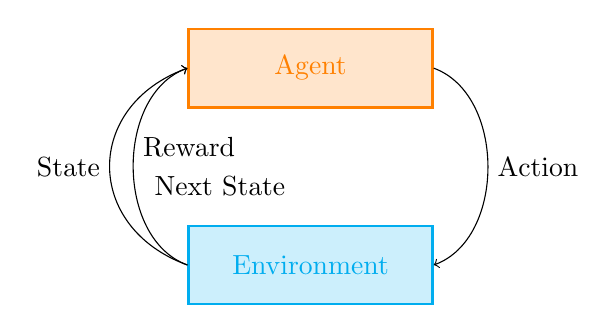
\begin{tikzpicture}[every node/.style=draw]
 \node[rectangle, 
 draw, 
 thick,
 minimum width = 3.1cm,
 minimum height = 1cm,
 color=cyan,
 fill=cyan!20] (A) at (0,0) {Environment};
 \node[rectangle, 
 draw, 
 thick,
 minimum width = 3.1cm,
 minimum height = 1cm,
 color=orange,
 fill=orange!20,
 ] (B) at (0,2.5) {Agent};

 \draw [->] (A.west) to [bend left=70] node [midway,right, draw=none, yshift=+2.5mm]{Reward} node[midway, yshift=-2.5mm,xshift=+11mm,draw=none]{Next State }(B.west);
 \draw [->] (A.west) to [bend left=70, min distance=1.4cm] node [midway,left, draw=none]{State} (B.west);
 \draw [->] (B.east) to [bend left=70] node [midway,right, draw=none]{Action} (A.east);
\end{tikzpicture}
\caption{Reinforcement learning model.}
\end{figure}
One unique challenge in reinforcement learning is balancing exploration and exploitation.
To succeed in a task, the agent must exploit actions that, through experience, have yielded the most rewards, although, 
to have experience and perform better in the future, the agent must explore new actions. 
The dilemma is that neither exploration nor exploitation can be pursued exclusively without failing at the task
\cite{reinforcement_learning}

 \subsection{Markov Decision Process}
 Reinforcement learning can be described using the Markov Decision Process(MDP). MDP is the final summary concept of the individual elements:
 \begin{itemize}
 \item The Markov Property 
 \item The Markov Decision Chain
 \item The Markov Reward Process
 \end{itemize}
 \subsubsection*{Markov Property}
 This means that the transition to state $t_{+1}$ from state {t} is independent of the past, meaning that our current state already captures all the relevant information from the past.
 Defined by the following equation:

 \begingroup
 \Large
 \begin{equation*}
 P(S_{t+1}|S_t) = P(S_{t+1}|S_1,...,S_t)
 \end{equation*}
 \endgroup
 \subsubsection*{Markov Decision Chain}
 A Markov chain is a mathematical system that experiences transitions from one state to another according to certain probabilistic rules. 
 The defining characteristic of a Markov chain is that no matter how the process arrives at its present state, the possible future states are fixed. 
 In other words, the probability of transitioning to any particular state is dependent solely on the current state.
 \begin{figure}[H]
 \centering
 \begin{tikzpicture}[every node/.style=draw]
 \node[circle, 
 draw, 
 thick,
 minimum width = 1.3cm,
 color=gray,
 fill=gray!20] (1) at (0,0) {$S1$};
 \node[circle, 
 draw, 
 thick,
 minimum width = 1.3cm,
 color=gray,
 fill=gray!20] (2) at (2.5,3) {$S2$};

 \node[circle, 
 draw, 
 thick,
 minimum width = 1.3cm,
 color=gray,
 fill=gray!20] (3) at (5,0) {$S3$};

 \draw [->, thick, -{Latex[length=3.5mm]}] (1.north) to [bend left=30] node [midway,left, draw=none]{0.4} (2.west);
 \draw [->, thick, -{Latex[length=3.5mm]}] (1.east) to [bend right=30] node [midway,yshift=-8 ,draw=none]{0.6} (3.west);
 \draw [<-, thick, -{Latex[length=3.5mm]}] (3.west) to [bend right=30] node [midway,yshift=8 ,draw=none]{0.3} (1.east);
 \draw [<-, thick, -{Latex[length=3.5mm]}] (3.north) to [bend right=30] node [midway,right ,draw=none]{0.7} (2.east);
 \draw [->, thick, -{Latex[length=3.5mm]}] (2.east) to [bend right=30] node [midway,left,draw=none]{0.5} (3.north);
 \draw [<-, thick, -{Latex[length=3.5mm]}] (2.west) to [bend left=30] node [midway,right, draw=none]{0.5} (1.north);


 \end{tikzpicture}
 \caption{Example of a Markov Decision Chain.}
 \end{figure}

 As can be observed by the example Markov Decision Chain, the transition probabilities are fixed and are only dependent on the current state, this is the Markov property.

 \begingroup
 \Large
 \begin{equation*}
 P(S_{t+1}|S_t)
 \end{equation*}
 \endgroup

 Definition of the probability of transitioning to any particular state given the current state.


 \subsubsection*{Markov Reward Process}
 As it suggests, the Markov Reward Process is a Markov process with the difference that it includes a reward system that indicates how much reward is accumulated through a particular sequence.
 An additional factor is applied, the \textbf{discount factor $\gamma$} that indicates how much the future reward is discounted. if $\gamma = 0$ 
 then the agent will only consider the immediate reward, if $\gamma = 1$ then the agent will consider all subsequent rewards. 
 In practice, these extreme values are ineffective, and $\gamma$ is usually set to values between 0.9 and 0.99

 \subsection{Bellman equation}
 As the agent moves through the Markov decision chain, one problem develops, how to choose the path that maximises future rewards from the current point onwards. 
 
 To solve this problem, a recursive equation is used, the Bellman equation.
 
 $V(s) = max_a (R(s,a)+\gamma V(s')) $ 
 
 The Bellman equation sums to the present reward the discount factor multiplied by the best next value output by the value function.

 The optimal value function $V^(s)$ maximises the expected reward. To achieve this, the Bellman equation is solved by iteratively updating the value function until $V^(s)$ is reached.

 % Q values are calculated using the Bellman equation, the Bellman equation takes the present reward and sums to it the discount factor multiplied by the best next q value of the combination of the next action and state

\section{Learning Algorithms}
One of the main decisions in implementing a reinforcement learning algorithm is the learning algorithm, to understand the algorithm decision its important to understand how this differ.
\begin{figure}[H]
\centering
\includegraphics[width=1\textwidth]{rl_algorightms.eps}
\caption{A non-exhaustive, but useful taxonomy of algorithms in modern RL from OpenAI\cite{openai_rl}.}
\label{fig:rl_algorightms}
\end{figure}

The first major split in RL algorithms is whether it is model-free or model-based. Model-based algorithms use a model of the environment, which is capable of mimicking its behaviour, this allows inferences to be made about how the environment will behave given an action and what the next reward will be. This reinforcement learning method is inadequate for the current problem due to the high complexity of the environment in which the agent is interacting, making it impossible to model it.

The second decision is between \textbf{policy optimization} and \textbf{Q-Learning}. 
While both approaches have similar concepts and are driven by MDP, they are internally different. 

In Q-learning, the goal is to determine a single action from a set of discrete actions by finding the action with the highest Q-value. While in policy optimisation, the goal is to learn a map from state to action, this can be stochastic and, as opposed to Q-Learning, works in continuous action spaces.

Q-Learning was a better fit for the problem in study as the action space was discretised. Apart from the action space, the Implementation of Q-learning is simpler and more common.

The algorithm decision was set on Deep Q-Network (DQN). The main difference between DQN and Q-Learning is that DQN implements a neural network replacing the Q-table. This is a benefit due to the complexity of the environment and the total number of possible states. Using standard Q-learning would require a very large q-table, which is a huge memory and computational burden.

\section{Training Framework}
Followed by the new advances in RL, there was a growing need for a common benchmarking framework that would allow for comparing algorithms and implementations.

The OpenAI team released Gym to enable this, by providing an accessible API and standardised environments. Gym is now the most widely used tool in RL research, it has a large community and documentation and a growing number of environments\cite{gym}.

Gym was chosen as the framework to standardise the implementation which allows for an easier understanding and comparison, beyond this, the Gym also facilitates the implementation by using all the pre-built functions\cite{openai}.

\section{Previous Implementations}
To develop this project it was important first to study previous implementations, what problems were faced and the reasoning behind their decisions, 
this brought light to many problems and details of implementing reinforcement learning, especially for walking.

One important implementation was the \textbf{Deep Q-Learning for Humanoid Walking}\cite{atlas_rl}, an implementation of reinforcement walking on the Atlas platform.
This implementation highlights some of the general pre-conceptions regarding the reward system and how to handle the complexity of controlling all the joints simultaneously.
%TODO: expand more explored implementations

\section{Logging and Reproducibility}
One of the most important aspects of machine learning and reinforcement learning is data logging and reproducibility. 
This project required extensive testing of hyperparameters and reward systems. 
To understand the results and their correlation with the variables in testing as well as being able to reproduce them, it is important to log all the hyperparameters and results.\linebreak
\textbf{Requirements for logging:}
\begin{itemize}[leftmargin=+0.5in]
 \item Hyperparameters
 \item Performance metrics
 \item Code
 \item Models
 \item Renderings
\end{itemize}
From previous experiences with machine learning and logging platforms, MLflow was the first option analysed. Although Weights \& Biases (WandB) was the chosen platform, WandB offered a hosted version option compared to MLflow. 
WandB also integrates with Keras allowing for a seamless implementation. WandB fills all the requirements and allows for a comparison of the renderings and performance results between runs.